% Activate the following line by filling in the right side. If for example the name of the root file is Main.tex, write
% "...root = Main.tex" if the chapter file is in the same directory, and "...root = ../Main.tex" if the chapter is in a subdirectory.
 
%!TEX root = TNTinderSee.tex 
%%%%%%%%%%%%%%%%%%%%%%%%%%%%%%% 80-Char line %%%%%%%%%%%%%%%%%%%%%%%%%%%%%%%%%%

\chapter{Ergebnisse}

\begin{figure}[htb]
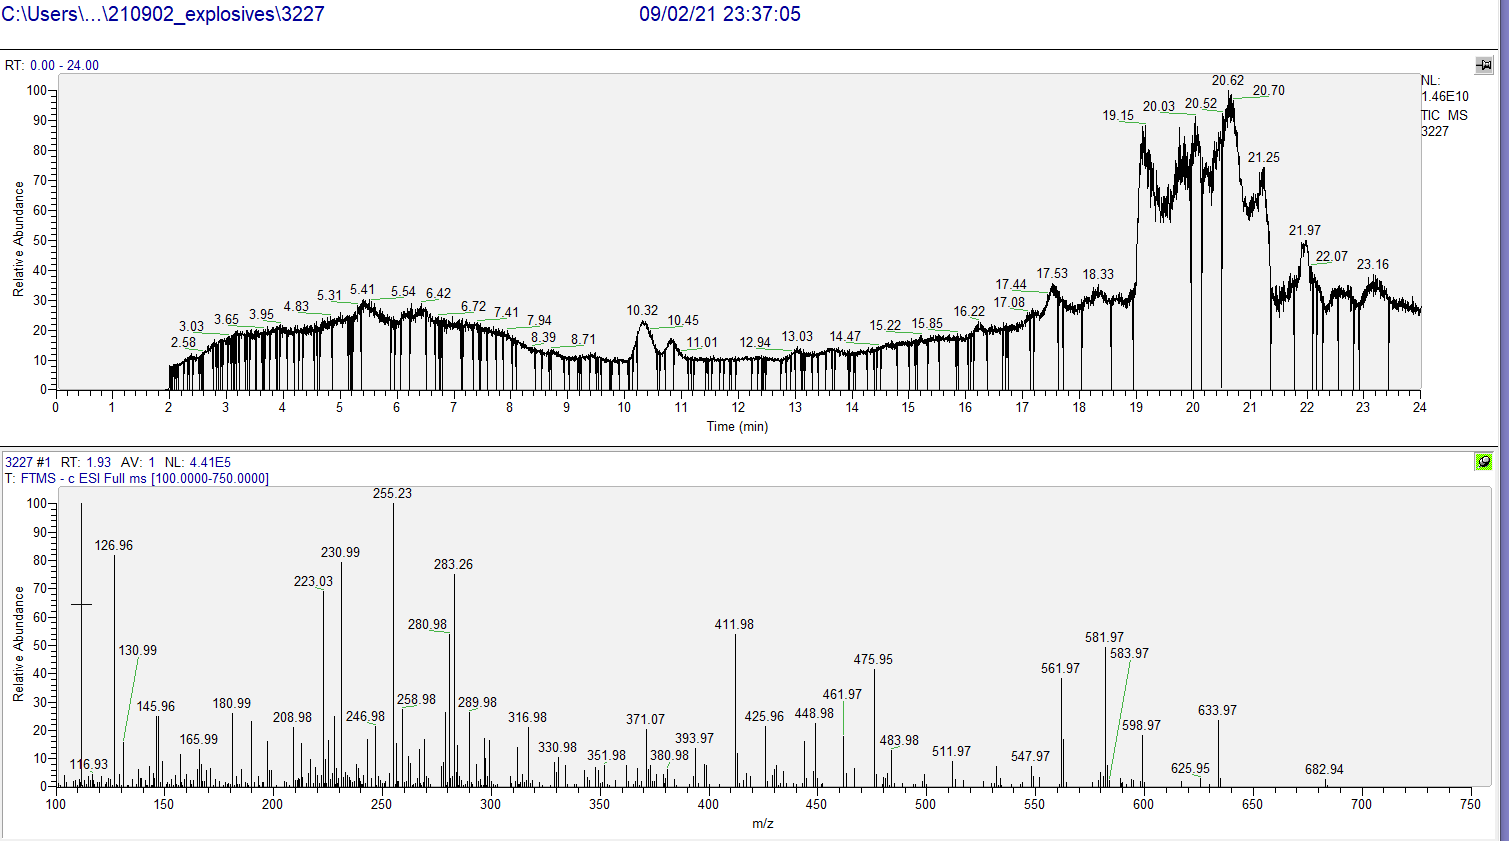
\includegraphics[height=\textheight,%
                   width=\textwidth,%
                   keepaspectratio]{Bilder/TIC_3227_SampleW1.PNG}
\caption{Total Ion Count W01 vom 19.07.2021}
\end{figure}
\begin{figure}[htb]
\includegraphics[height=\textheight,%
                   width=\textwidth,%
                   keepaspectratio]{Bilder/TIC_5ppbSTandard.PNG}
\caption{Total Ion Count - Referenzstandard}
\end{figure}
\begin{figure}[htb]
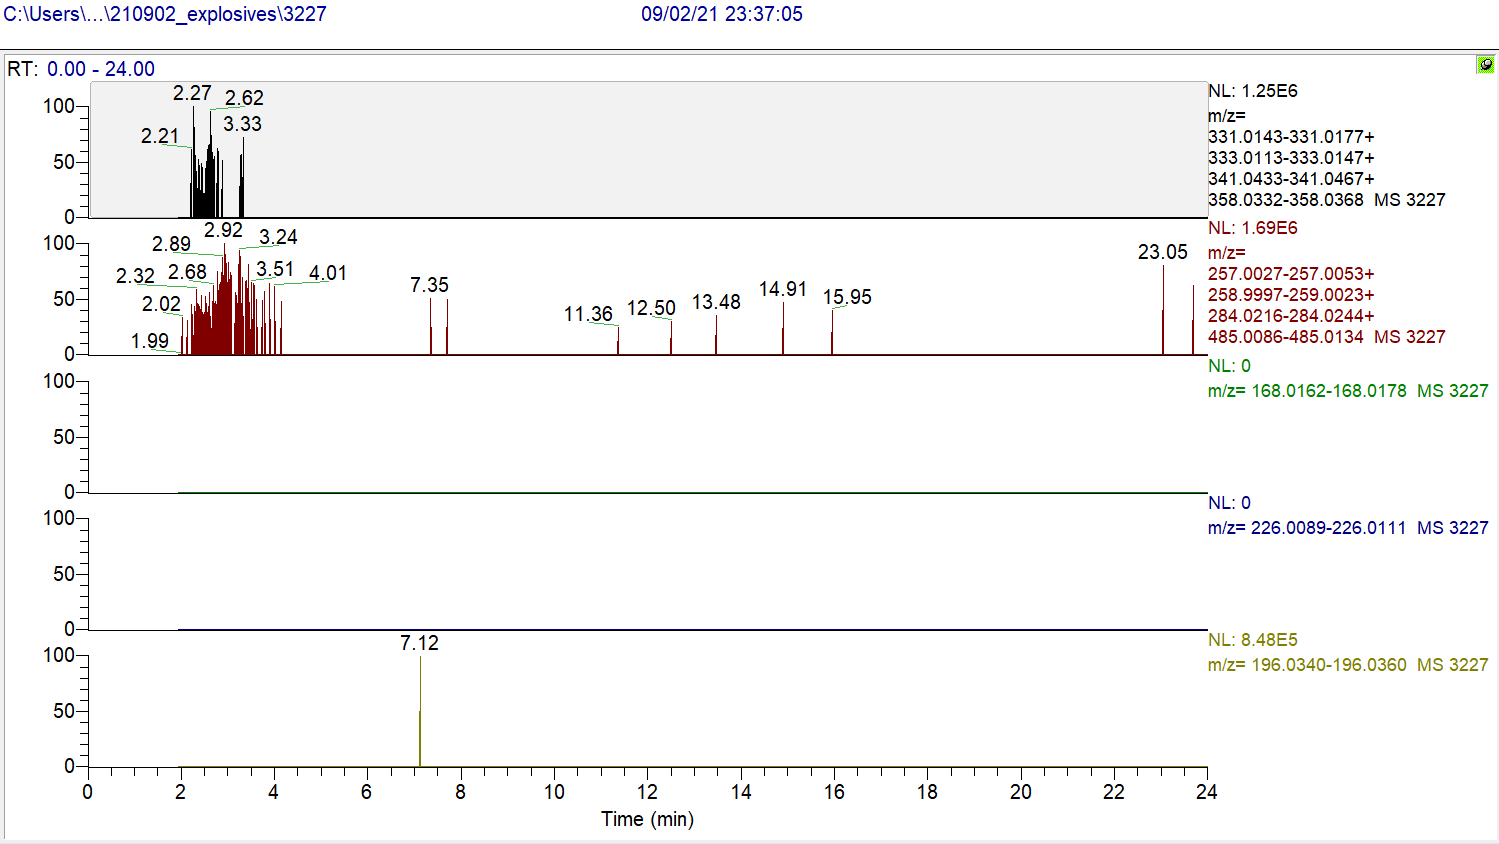
\includegraphics[height=\textheight,%
                   width=\textwidth,%
                   keepaspectratio]{Bilder/Explosives_3227_SampleW1.PNG}
\caption{Chromatografieergebnis mit Focus auf sprengstofftypische Verbindung. Von oben nach unten: HMX (schwarz), RDX (grün), TNT (blau), ADNT (gelb)}
\end{figure}
Es gibt zwei Spitzen für 4-ADNT und 2-ADNT-Isomere.
Was bedeuten die Spitzen bei HMX und RDX?

\begin{figure}[htb]
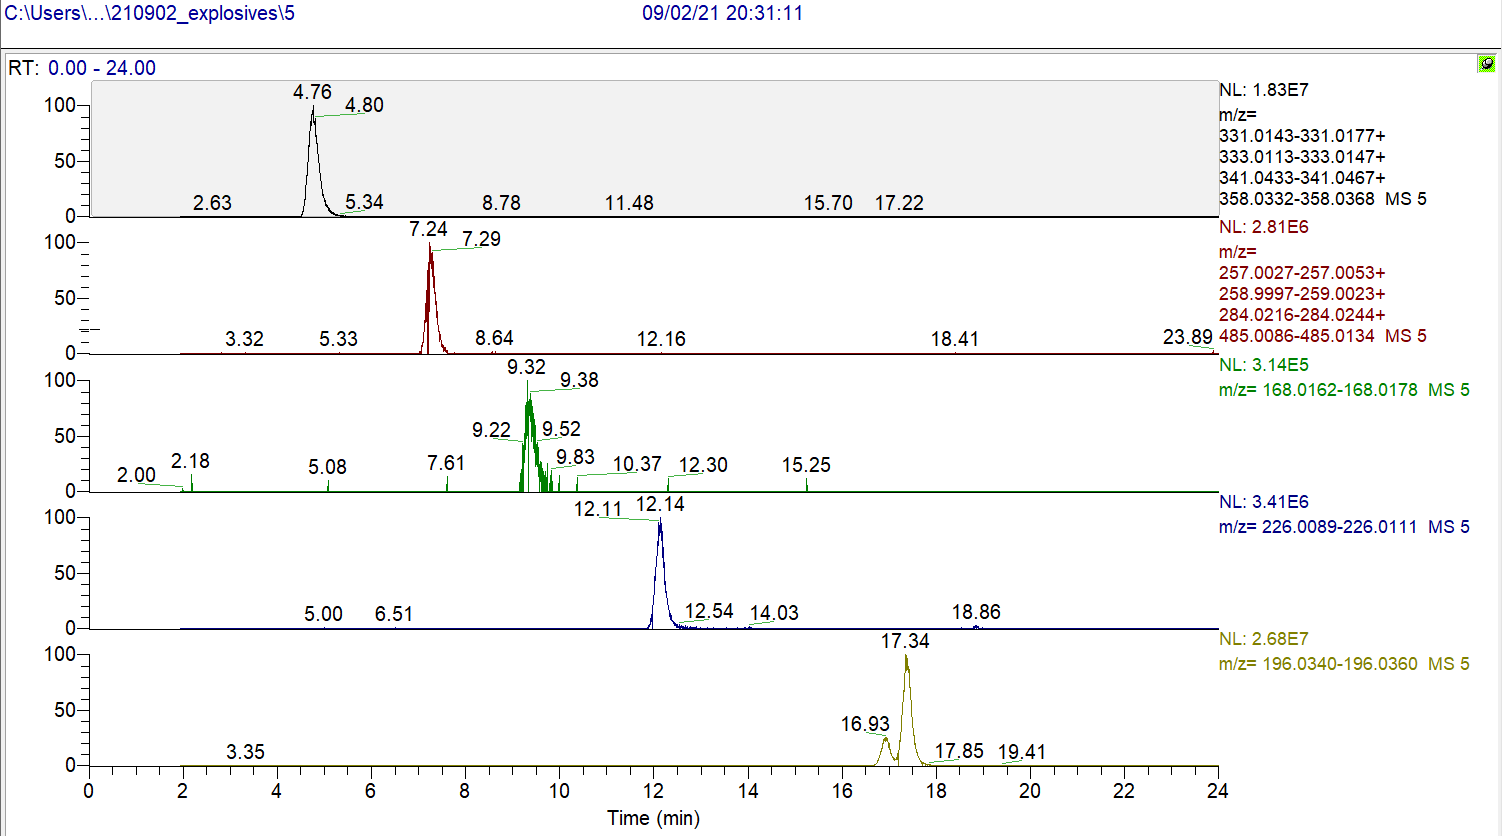
\includegraphics[height=\textheight,%
                   width=\textwidth,%
                   keepaspectratio]{Bilder/Explosives_5ppb.PNG}
\caption{Vergleichende Standardwerte}
\end{figure}
\begin{figure}[htb]
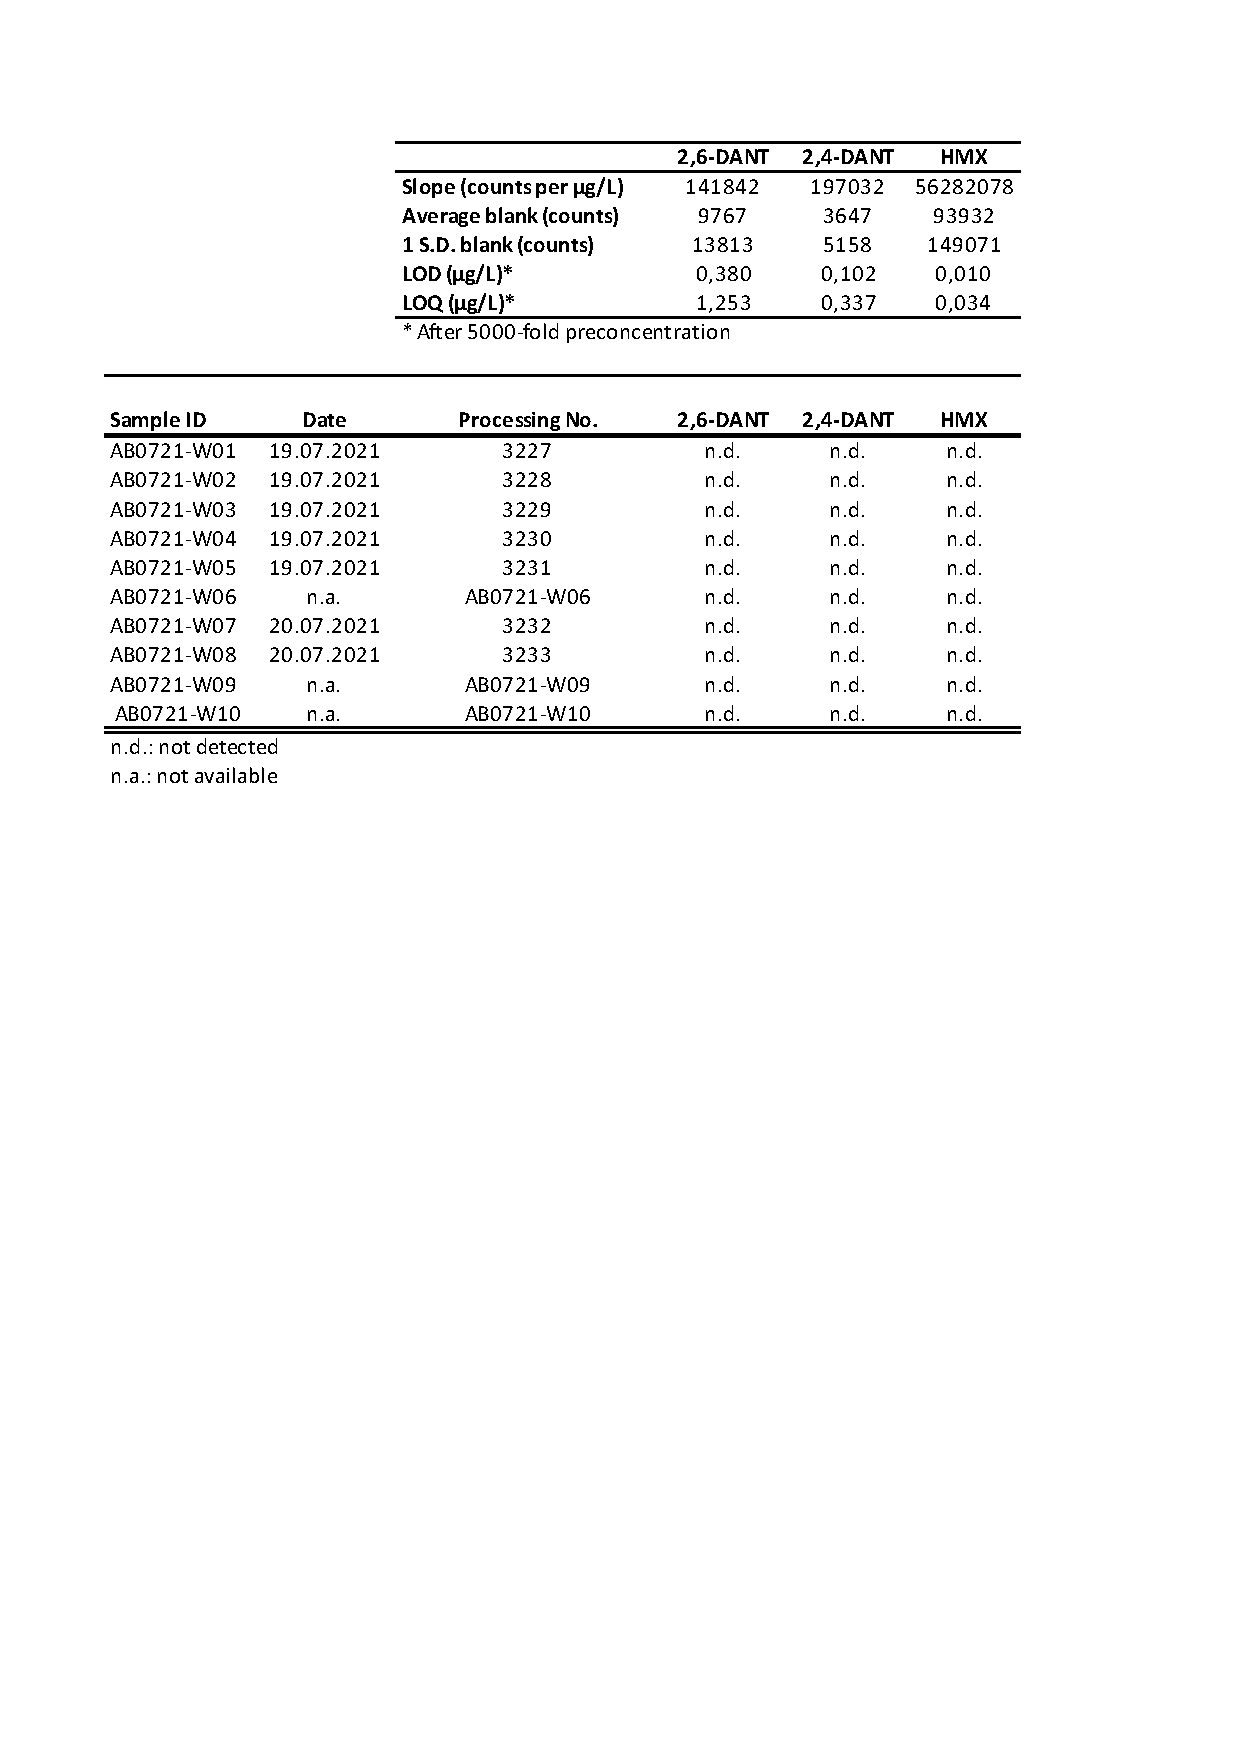
\includegraphics[height=\textheight,%
                   width=\textwidth,%
                   keepaspectratio]{Bilder/MC_data_Aldebaran.pdf}
\caption{Datensatz}
\end{figure}
\section{Diskussion der Ergebnisse}
Wir können Entwarnung geben: Das von uns abgesuchte Gebiet ist unbelastet. Ein
solches Ergebnis ist zwar unspektakulär, jedoch auch erleichternd. Wieso 
unsere Proben keine Spuren von Sprengstoffen oder deren Zerfallsprodukten 
enthalten ist eine andere Frage, möglicherweise wurden sie seit dem xx.xx.xxxx%TODO: DATUM
von der Organik vor Ort aufgenommen, und uns bei der Probenfiltrierung
abhanden gekommen. Auf jeden Fall sollten weitere Untersuchungen (vorzugsweise
an Bord der ALDEBARAN) stattfinden, sowie evtl. neue Methoden zur Erfassung
von Sprengstoffen in Organik entwickelt werden.
